\scanpage{24}\mspage{23}
b) $\Rightarrow$ a) If $F'$ is a refinement of $G$ such that $F'$ subfigure of $F$, we have $|F|\subset|F'|\subset|G|$, and since $|F|=|G|$ we
have $|F|=|F'|$, hence $F=F'$, since $F$ subfigure of $F'$,
% slanted
\margin{\uline{Let us also give} equ\unsure{ivalent|ivalent} condition c) \inserted{$F\ll G$ and} Every stratum of $G$ is a union of strata of $F$. And when \unsure{we no longer assume|we do not assume} \unsure{in advance|in advance} that $F\ll G$, condition d) \[\left\{\begin{aligned}&1^\circ)\ \text{Every stratum of }G\text{ is a union of strata of }F\\&2^\circ)\ \forall \deleted{\unsure{B}}A\in F,\quad G^A=\{B\in G\mid B\supset A\}\text{ has a}\\&\text{least element.}\end{aligned}\right.\]}

a) $\Rightarrow$ b) Suppose that $|F|\ne|G|$, \deleted{let $x\in|G|\setminus|F|$, consider the} There therefore exists a figure $\deleted{F}H$ \deleted{which is} \inserted{such} that \deleted{\unsure{empty}, which is a refinement of $G$,}
\[ \left\{\begin{aligned} &|H|\ne\varnothing\\ &\deleted{F}H\ \text{refines }G\\ &\deleted{F}H\ \text{disjoint from }F \end{aligned}\right. \]
for example we take \unsure{an} $x\in|G|\setminus|F|$, and the figure $\deleted{F}H=\{\{x\}\}$. Now we have

\uline{Corollary}\enspace Let $F,H$ be two figures which refine $G$, and such that $F$ and $H$ \deleted{disjoint} \inserted{compatible}. Then $F\cup H$ refines $G$.
% slanted
\margin{\figure{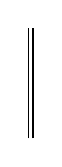
\begin{tikzpicture}\draw (0,0)--(0,1.4) (.06,0)--(.06,1.4);\end{tikzpicture}} to be noted \unsure{as|as an|this} \unsure{interesting|interesting} formal property. \unsure{Contrary case|On the contrary|On the other hand} $\pm$ \unsure{general} \unsure{(at least|(to the neighbour}, the \unsure{tame|tame} \unsure{construction|opposites|conditions}) of unions (non-tame case) if $F$ and $G$ disjoint\ldots}
\inserted{\uline{More generally}, it works for \unsure{arbitrary|arbitrary} Sup (in the sense of $\leq$)}
Indeed, we use the fact that the multistrata of $F\cup H$ are the multistrata \deleted{which are common to $F$} which belong to $F$, or \deleted{to} $H$. Now the refinement property is checked on the multistrata.

\uline{Definition} We then say that $F$ is a \inserted{\uline{subdivision}} of $G$.
